%!TEX root=SpGEMM_ACCUMULO_HPEC.tex

\section{TableMult Design}
\label{sDesign}


\subsection{Matrix Multiplication}
Given input matrices $\matr{A}$ of size $n \times m$, $\matr{B}$ of size $m \times p$,
and operations $\oplus$ and $\otimes$ for scalar summation and multiplication,
the matrix multiplication $\matr{A} \,{\oplus}.{\otimes}\, \matr{B} = \matr{C}$, or more shortly $\matr{A}\matr{B} = \matr{C}$,
defines the entries of result matrix C as 
\[ \matr{C}(i,j) = \bigoplus_{k=1}^m \matr{A}(i,k) \otimes \matr{B}(k,j) \]
We call intermediary results of $\otimes$ operations \emph{partial products}.

In the case of sparse matrices, we only perform $\oplus$ and $\otimes$ operations where both operands are nonzero,
an optimization stemming from the requirement that 0 is an additive identity of $\oplus$ such that $a \oplus 0 = 0 \oplus a = a$,
and that 0 is a multiplicative annhilator of $\otimes$ such that $a \otimes 0 = 0 \otimes a = 0$.
Sparse arithmetic is impossible without these conditions, since in that case zero elements could generate nonzero results.

In Accumulo, zero elements are entries that do not exist in a table. Entries that actually contain the value zero may exist
from an operation producing a zero value (such as summing partial products 5, -3 and -2).  
We currently deliver no special treatment to these entries and plan on adding
an optional feature that removes them when encountered.

There are two general patterns for performing matrix multiplication: inner product and outer product.
We study each in terms of how it implements the $\otimes$ component of matrix multiplication,
deferring the $\oplus$ operation to run on output generated from applying $\otimes$.
In the pseudocode, `:' stands for ``all positions'' in the spirit of Matlab notation.

The more common inner product method runs the following:
\begin{algorithm}[h]
\SetKwBlock{fore}{for}{} 
\SetKw{emit}{emit}
\fore($i = 1\col n$){
\fore($j = 1\col p$){
\emit{$\matr{A}(i,:) \cdot \matr{B}(:,j)$}
}}
\end{algorithm}

\noindent where the operation $\cdot$ is inner (also called dot) product on vectors, which we may unfold as
\begin{algorithm}[h]
\SetKwBlock{fore}{for}{} 
\SetKw{emit}{emit}
\fore($i = 1\col n$){
\fore($j = 1\col p$){
\fore($k = 1\col m$){
\emit{$\matr{A}(i,k) \otimes \matr{B}(k,j)$}
}}}
\end{algorithm}

Inner product has an advantage of generating output ``in order,'' meaning that all partial products needed 
to compute a particular element $\matr{C}(n,p)$ are generated consecutively by the third-level for loop.
We may apply the $\oplus$ operation immediately after each third-level for loop and obtain an element in the result matrix.
This means that inner product is easy to ``pre-sum,'' an Accumulo term for applying a Combiner
locally before sending entries to a remote but globally-aware table combiner.
% move to another section?
%Inner product also generates output ``in order'' in a second sense: 
It is also adventageous that inner product generates entries sorted by row 
and column, which allows inner product to be used in standard iterator stacks that require sorted output.

Despite its order-preserving advantages, we chose not to implement inner product 
because it requires multiple passes:
the second-level for loop that scans over all of input matrix $\matr{B}$
repeats for each row of $\matr{A}$ from the top-level for loop iteration.
%The same effect holds if we flipped the process symmetrically.
Under our assumption that we cannot fit $\matr{B}$ entirely in memory,
multiple passes over $\matr{B}$ translates to multiple Accumulo scans that each require a disk read.
We found in our performance tests that multiple scans over $\matr{B}$ 
delivered over an order of magnitude worse performance, taking over 100 seconds to multiply SCALE 11 inputs
whereas the outer product method ran in under 8.

Outer product matrix multiply runs the following:
\begin{algorithm}
\SetKwBlock{fore}{for}{} 
\SetKw{emit}{emit}
\fore($k = 1\col m$){
\emit{$\matr{A}(:,k) \times \matr{B}(k,:)$}
}
\end{algorithm}

\noindent where the operation $\times$ is outer (also called tensor or Carteisan) product on vectors, which we may unfold as
\begin{algorithm}
\SetKwBlock{fore}{for}{} 
\SetKw{emit}{emit}
\fore($k = 1\col m$){
\fore($i = 1\col n$){
\fore($j = 1\col p$){
\emit{$ \matr{A}(i,k) \otimes \matr{B}(k,j)$}
}}}
\end{algorithm}

Outer product emits partial products in chaotic, unsorted order.
This is due to moving the $i$ and $j$ for loops, both responsible for determining partial product position,
below the top-level $k$ for loop.

On the other hand, outer product only requires a single pass over both input matrices.
This is because the top-level $k$ for loop fixes a dimension of both matrix $\matr{A}$ and $\matr{B}$.
Once we finish processing a full column of $\matr{A}$ and row of $\matr{B}$, the column and row are finished;
there is no need to read them again (i.e., we never need to restart the top-level for loop).

We may speed the outer product algorithm by storing rows of table $\matr{B}$ in memory,
which eliminates the need to re-read rows of $\matr{B}$ for each run of the third-level for loop.
%Storing one row in memory is a much lower cost than storing a whole matrix in memory.
In the case of Accumulo, we can even eliminate the need to hold a row in memory by using
deepCopy SKVI methods to store ``pointers'' to the beginning of the current row m of table $\matr{B}$.
However, this strategy may come at the cost of extra disk seeks, and so
we leave testing its performance to future work, for now storing the current row of table $\matr{B}$ in memory.

Since m is the second dimension of matrix $\matr{A}$, we implement 
SpGEMM to operate on the transpose $\matr{A^\tr}$ of input table $\matr{A}$.



\subsection{TableMult Iterators}
We use three new server-side iterators to implement SpGEMM: 
RemoteSourceIterator, TwoTableIterator and RemoteWriteIterator.
We place these iterators on a scan of Table $\matr{B}$. 
%The scan itself emits no entries except for a smidgeon of ``monitoring entries'' 
%that inform the client about TableMult progress. 
%% Instead, the scan on table $\matr{B}$ reads from table $\matr{A}$T
%% by opening a Scanner and writes to result table $\matr{C}$
%% by opening a BatchWriter, all within the scan's iterator stack.
%% See Figure~\ref{fIteratorStackSpGEMM} for an illustration.

The key idea behind the TableMult iterators is that they divert normal dataflow by opening a BatchWriter,
%reducing entries sent to the client to zero and instead sending 
redirecting entries out-of-band to a sink table via %result table $\matr{C}$
Accumulo's standard ingest channel that does not require sorted order. 
The scan itself emits no entries except for a smidgeon of ``monitoring entries'' 
that inform the client about TableMult progress.
%Thus the TableMult iterators act as reduction iterators, even though they actually transmit 
%a huge stream of entries out-of-band to another Accumulo table.
We also enable multi-table iterator dataflow by opening Scanners 
that read outside Accumulo tables out-of-band.
%which in the case of SpGEMM means scanning table $\matr{A^\tr}$.
Scanners and BatchWriters are standard tools for Accumulo clients; 
by creating them inside Accumulo iterators, we enable all the functionality of client-side processing 
within the Accumulo server.

In the case of SpGEMM, we use a Scanner on table $\matr{A^\tr}$
and a BatchWriter on result table $\matr{C}$.
Figure~\ref{fIteratorStackSpGEMM} illustrates TableMult's data flow.

\begin{figure}[htb]
\centering
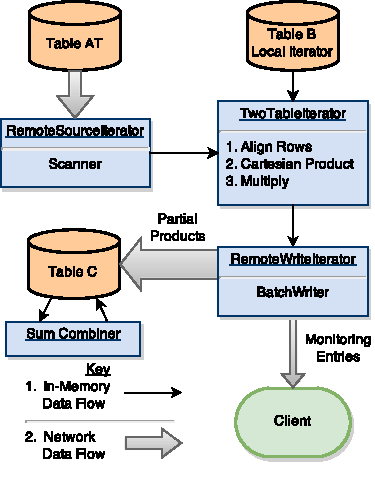
\includegraphics[width=3.3in]{TableMultIteratorStack}
\caption{Data flow through the TableMult iterator stack}
\label{fIteratorStackSpGEMM}
\end{figure}

\subsubsection{RemoteSourceIterator}
RemoteSourceIterator contains a Scanner that scans an Accumulo table
(not necessarily in the same cluster) with the same range it is seeked to.
Clients pass connection information including zookeeper hosts, timeout,
username, and password to a RemoteSourceIterator via iterator options
in the form of a \texttt{Map<String,String>}.

A client may also specify rows and columns to scan via a rowRanges and colFilter option, 
if not scanning the whole table. We encode the rowRanges option in ``D4M syntax,'' consisting of 
delimitted row keys and the `:' character to indicate ranges between row keys.
In our encoding, ``a,:,b,d,f,:,'' translates to the ranges 
``[a,b\textbackslash{}0), [d,d\textbackslash{}0), [f,$+\infty$).'' The comma used as a delimitter in the example 
may be any character not present in a row key, and we disallow rows consisting of a single `:'.
We do not include column family or deeper fields in our encoding and leave them empty, 
which is ok for our purpose since SpGEMM operates on the Cartesian product of entire rows.

ColFilter is defined similarly to rowRanges, except that we do not allow ranges to occur in the colFilter
because Accumulo does not index columns.  We may enable ranges anyway in the future by using an Accumulo
Filter iterator subclass to only return the entries within a column range set.
Such a feature would require scanning every column, 
which can affect performance if bottlenecked on table reads.
We encourage users to maintain a tranpose table for cases requiring column indexing.

Scanning a subset of rows in a table is crucial for queued analytics, since those analaytics 
operate on a graph subset.  However, for simplicity of performance evaluation, 
our experiments in Section~\ref{sPerformance} multiply whole table inputs.

\subsubsection{TwoTableIterator}
TwoTableIterator reads from two iterator sources, one for $\matr{A}$T and one for $\matr{B}$,
and performs the core operations of the outer product algorithm in three phases:
\begin{enumerate}
\item Align Rows.  Read entries from table $\matr{A^\tr}$ and $\matr{B}$ until they reside at the beginning of a matching row
or until one runs out of entries. We skip non-matching rows as they would be multiplied by an all-zero row in the
opposite table and generate all zero patrial products.
\item Cartesian product. Read both matching rows into an in-memory data structure. 
Initialize an iterator that emits pairs of entries from the the matching rows' Carteisan product.
\item Multiply. Pass pairs of entries to $\otimes$ and emit results. 
\end{enumerate}

In implementing the $\otimes$ operation as ordinary real number multiplication and $\oplus$ as addition,
we decode Accumulo value byte arrays into Strings and then into \texttt{java.math.BigDecimal}
objects. BigDecimal enables multiplication to work for very large and very precise real-valued numbers,
though it may be cumbersome for small integer multiplication. We use BigDecimal anyway since 
writing result entries is our bottleneck, not iterator processing.
%found writing data using a BatchWriter to be our primary bottleneck 

\subsubsection{RemoteWriteIterator}
RemoteWriteIterator writes entries to a remote Accumulo table using a BatchWriter created on \texttt{init}.
Entries do not have to be in sorted order because Accumulo sorts incoming entries as part of its
standard ingest process. Like RemoteSourceIterator, the client passes connection information 
for the remote table via iterator options.

Barring extreme events such as exceptions in the iterator stack or thread death,
we designed RemoteWriteIterator to maintain correctness, such that entries generated from
RemoteWriteIterator's source will be written to the remote table once.
One way to accomplish this is by performing all BatchWriter operations within a single function call
before ceding thread contol back to the Accumulo tablet server.  We do this in the \texttt{seek} method,
streaming every entry from RemoteWriteIterator's source (within the seek range) into a BatchWriter at once, 
by repeatedly calling the \texttt{getTop} and \texttt{next} methods of its source and \texttt{flush}ing afterward.

% Not too important but a common concern from some in the Accumulo community:
We completely close the BatchWriter in a finalize method.
The JVM does not guarantee calling objects' finalize method before it garbage collects them, 
but in our experience, the JVM called finalize in every non-extreme circumstance
and we guarantee correctness even if finalize is not called. Alternatives such as using \texttt{java.lang.ref}
classes and closing BatchWriters in place of flushing them are open.
% link: http://books.google.com/books?id=ka2VUBqHiWkC&pg=PA27&lpg=PA27&dq=effective+java+avoid+finalizers&source=bl&ots=yYGkMgn-QZ&sig=o66EY94GVzB3uvNOvj9eLhdI35k&hl=en&sa=X&ei=0nsxUPeHHILp0gHx1oBI&ved=0CGMQ6AEwAg#v=onepage&q=effective%20java%20avoid%20finalizers&f=false

A performance concern remains in the case of TableMult over a subset of the input tables' rows 
that consists of many disjoint ranges, such as 1M ``singleton'' ranges spanning one row each.
It is inefficient to flush the BatchWriter before returning from each seek call, which happens once per 
disjoint scan range, and a known Accumulo issue could even crash the tablet server \cite{ACCUMULO-3710}.
In order to accomodate this case, we ``transfer seek control'' over the desired row range
subset from the Accumulo tablet server to the RemoteWriteIterator by passing the range objects through 
iterator options encoded as a D4M range string (see above), as opposed to the usual method of 
passing range objects to the \texttt{setRanges} BatchScanner method for table $\matr{B}$.
The RemoteWriteIterator can then traverse all ranges in the desired subset before returning from a seek.
In the case of multiple tablets for table $\matr{B}$, the RemoteWriteIterator running on each tablet handles 
the portion of ranges that intersects with the range of keys in its tablet.

We include an option to BatchWrite the result table's transpose in place of or alongside
the result table. Writing the transpose enables maintenance of transpose indexing for those using the 
D4M Schema \cite{kepner2013d4m}, as well as facilitating chaining TableMults one after another.

\subsubsection{Lazy $\oplus$}
We lazily perform the $\oplus$ portion of matrix multiplication (i.e., summing partial products)
by placing a Combiner subclass implementing $\oplus$ logic on the result table at scan, minor and major compaction scopes.
Thus, $\oplus$ occurs sometime after the RemoteWriteIterator writes partial products to the result table,
yet necessarily before any entry from the result table may be seen such that we always achieve correctness.
This could happen in part when Accumulo flushes the result table to a new RFile, when Accumulo compacts RFiles 
together, or when a client scans the result table. 

The key algebraic requirement for implementing $\oplus$ inside a Combiner
is that $\oplus$ must be associative and commutative.
These properties allow us to perform $\oplus$ on subsets of a result element's partial products 
and on any ordering of them, which is chaotic by the outer product's nature.
If we truly had an $\oplus$ operation that required seeing all partial products at once,
we would have to either gather partial products at the client or initiate a full major compaction.

Our choice to defer the $\oplus$ operation 

\subsubsection{Monitoring}
RemoteWriteIterator never emits entries to the client by default. 
One downside of this approach is that clients cannot precisely track the progress of a TableMult operation.
The only information clients would have are scan and write rates from the Accumulo monitor,
whether a scan is running, idle or queued from the tablet server, and what partial products 
are written to the result table so far from scanning the result table.

We therefore implemented a monitoring option on RemoteWriteIterator that occassionally emits entries
back to the client at ``safe'' points in the middle of a TableMult, that is,
at points when the iterator stack may recover its state if Accumulo destroys, later re-creates and re-seeks it
to a range starting at its last emitted key (exclusive).
Stopping after emitting the last value in the outer product of two rows is naturally safe, since we may place that row key
in the emitted monitoring key and know, in the event of an iterator stack rebuild, to proceed to the next matching rows.
We are also experimenting with an encoding that permits stopping in the middle of an outer product by encoding the 
column family and qualifier of the rows in the outer product in the emitted monitoring key.

We control the frequency of emitting monitoring entries by specifying iterator options in terms of how many entries
before emitting or how long a duration between emitting monitor entries. We encode the number of entries processed so far 
in the monitoring entry value. Between the key and value, the client can see how far the TableMult operation progressed
in terms of number of emitted entries and progress in scanning row keys from tables $\matr{A^\tr}$ and $\matr{B}$.
%The approach scales as further B is split into more and more tablets.

In order for the client to receive monitoring entries before the TableMult completes,
we must change the \texttt{table.scan.max.memory} paramter of table $\matr{B}$ to as small a value as possible, say one byte. 
This forces Accumulo to send entries from the BatchWriteIterator to the client immediately as they are generated.
We may restore the previous parameter value (default 512KB) once the TableMult compeletes.
If a proposed change \cite{ACCUMULO-261} is applied to future Accumulo versions,
we will be able to change the tablet server scan cache on a per-scan basis rather than a per-table basis
that affects concurrent scans on table $\matr{B}$.
%not in this paper: gather information within the RemoteWriteIterator to send back to the client


\todo[inline]{Put Java signature of TableMult call?}

